%%%%%%%%%%%%%%%%%%%%%%%%%%%%%%%%%%%%%%%%%%%%%%%%%%%%%%%%%%%%%
% This template is a translation by Andreas Almqvist of the 
% Swedish Overleaf report template: "Luleå University of 
% Technology lab report template (TVM department)", which was
% authored by Magnus Gustafsson and colleagues at Luleå 
% University of Technology. If you have any comments or 
% requests, please get in touch with Andreas Almqvist, see
% https://bit.ly/almqvist
%%%%%%%%%%%%%%%%%%%%%%%%%%%%%%%%%%%%%%%%%%%%%%%%%%%%%%%%%%%%%

%%%%%%%%%%%%%%%%%%%%%%%%%%%%%%%%%%%%%%%%%%%%%%%%%%%%%%%%%%%%%
% - PREAMBLE                                              - %
%%%%%%%%%%%%%%%%%%%%%%%%%%%%%%%%%%%%%%%%%%%%%%%%%%%%%%%%%%%%%
% In the "Preamble" you define how the document should be formatted.
% Since LaTeX is a programming language that is compiled, you need
% to have a syntax that allows you to enter comments that are not
% interpreted by the compiler. By now, you have probably already
% realized that in LaTeX, you do this by starting with a percentage sign.

\documentclass[a4paper]{article}
% "\usepackage{}" loads packages that control formatting and make
% useful commands available.
\usepackage[margin=2cm]{geometry} % Change margins
\usepackage[utf8]{inputenc} % Character encoding - use this one.
\usepackage[T1]{fontenc} % Font encoding
\usepackage[english]{babel} % To write in English
\usepackage{graphicx} % Image handling
\usepackage{float} % For positioning of figures and tables
\usepackage{subcaption} % To refer to individual subfigures
\usepackage{xcolor} % For different colours
\usepackage{pgfplots} % For intrinsic LaTeX plotting
\pgfplotsset{compat=1.18} % Set the compatibility mode
\graphicspath{{Images/}} % Relative path to images. In this case,
% a folder called "Images".
\usepackage{caption} % Figure and table captions
\usepackage{mathtools, amsmath, amssymb} % Mathematics tools
\usepackage{siunitx} % Package for numbers, units, and ranges.
% Ex. \num{1e6}, \SI{15.3}{Nm}, and \SIrange{10}{20}{\celcius})
\sisetup{output-decimal-marker={.},range-phrase=--,
range-units=single,exponent-product=\cdot}
% If writing in Swedish, change to: output-decimal-marker={,}
\usepackage{verbatim} % Long comments, programming code, etc.
\usepackage{hyperref} % Hyperlinks
%\hypersetup{bookmarksopen=true, bookmarksopenlevel=0,
% linkcolor={blue}}

% For referencing, you can use the "biblatex" package
% Numerical references are done by:
%\usepackage[backend=bibtex,style=numeric,bibencoding=ascii]{biblatex}
%\usepackage[maxnames=6]{biblatex}
\usepackage[square, numbers, sort&compress]{natbib}
% APA references:
% \usepackage[style=apa,backend=biber]{biblatex}
% \DeclareLanguageMapping{swedish}{swedish-apa}
% The references are to be included in the "Bibliography".
%\addbibresource{references.tex} % This command specifies
% the file where the references of the "bibtex" type
% have been collected.

% Since LaTeX is a programming language, it can be
% useful to structure the document with comments.
% You can also create a main document and then include 
% different sections written in separate files.
% This is done using the command \import{Result.tex}

% In LaTeX, you can also define your own commands. The ones
% listed below are meant to simplify working with partial
% differential equations.
\newcommand{\p}{\partial} % "Curly" d in a partial derivative
\newcommand{\pde}[2]{\frac{\p #1}{\p #2}}
\newcommand{\pdetext}[2]{\p #1 / \p #2}
\renewcommand{\div}{\nabla\cdot}

%%%%%%%%%%%%%%%%%%%%%%%%%%%%%%%%%%%%%%%%%%%%%%%%%%%%%%%%%%%%%%
% -                         Title                          - %
%%%%%%%%%%%%%%%%%%%%%%%%%%%%%%%%%%%%%%%%%%%%%%%%%%%%%%%%%%%%%%
% The title page should not be numbered. The pages that receive
% a page prefix on each page are: preface, abstract,
% table of contents, and nomenclature. Starting from
% the introduction, page numbers are used.
%
% Page numbers are printed on each page, centred
% in the footer. Note that page numbering has already been
% done in this template.

% Images on the first page are best placed in the "author"
% command.

% Specify the author, email, and publication date.
% The title page can also include a figure to attract
% the reader to read the report.

% Of course, the content of the figure must be related to
% the work described in the report.

% A title can have high expectations. The title should be clear
% and descriptive, functioning as a mini-summary of
% the work. The reader should understand what the report is about
% by reading the title. However, the title should be short, 4-12 words,
% and should not contain formulas, abbreviations, or
% special symbols.

% A good title is one that accurately describes the content
% of the report with the fewest possible words. Sometimes,
% it can be practical to have a title and a subtitle.

% For laboratory reports include the email and lab instructor.

% Change the LTU logo for an English report.

%%%%%%%%%%%%%%%%%%%%%%%%%%%%%%%%%%%%%%%%%%%%%%%%%%%%%%%%%%%%%%
% - Document - %
%%%%%%%%%%%%%%%%%%%%%%%%%%%%%%%%%%%%%%%%%%%%%%%%%%%%%%%%%%%%%%
% The "document" section is where the actual text is
% written. You can divide the text into different sections.
% If you do this, LaTeX can generate a table of contents,
% headers, etc.
\title{A \LaTeX\ Template Presenting:\\ % \\ <-Inserts a line break
       A Guide for Writing Reports}

\author{
    \includegraphics[width=0.6\textwidth]{Images/hund_liten.jpg} \\
    \\
    \\
    {Author} \\
    {\tt author@student.ltu.se} \\
    {Department of Engineering Sciences and Mathematics} \\
    \\ 
    \includegraphics[width=0.2\textwidth]{Images/LTU_eng.jpg}
    }

\date{\today} % Prints today's date

\begin{document}

\maketitle % Generates title
\thispagestyle{empty} % Declares page style
%%%%%%%%%%%%%%%%%%%%%%%%%%%%%%%%%%%%%%%%%%%%%%%%%%%%%%%%%%%%%%
% -             PREAMBLE ENDS HERE                         - %
%%%%%%%%%%%%%%%%%%%%%%%%%%%%%%%%%%%%%%%%%%%%%%%%%%%%%%%%%%%%%%

%%%%%%%%%%%%%%%%%%%%%%%%%%%%%%%%%%%%%%%%%%%%%%%%%%%%%%%%%%%%%%
% -               Summary/Abstract                         - %
%%%%%%%%%%%%%%%%%%%%%%%%%%%%%%%%%%%%%%%%%%%%%%%%%%%%%%%%%%%%%%
\newpage % Each main heading: \section{} should start on a new page.
\pagenumbering{roman}

% Summary is called Abstract in English
\section*{Abstract} % "*" removes numbering from the title
The abstract is independent of the rest of the report. It should be possible to read the abstract without having read the report, and vice versa. The abstract should contain a brief description of the problem, method, the most important results, and their implications. It should be complete, objective, and easy to understand. The abstract should summarise the work, and any additional information that is not present in the report should not be included. The abstract should be concise and should contain a maximum of \numrange{150}{200}{} words. It should not include images or figures. It should not contain references or formulas, but it should describe the most important results.

%%%%%%%%%%%%%%%%%%%%%%%%%%%%%%%%%%%%%%%%%%%%%%%%%%%%%%%%%%%%%%
% -              Table of Contents                         - %
%%%%%%%%%%%%%%%%%%%%%%%%%%%%%%%%%%%%%%%%%%%%%%%%%%%%%%%%%%%%%%
\newpage % New page
\tableofcontents % Automatically generates a table of contents

%%%%%%%%%%%%%%%%%%%%%%%%%%%%%%%%%%%%%%%%%%%%%%%%%%%%%%%%%%%%%%
% -          Notations/Nomenclature                        - %
%%%%%%%%%%%%%%%%%%%%%%%%%%%%%%%%%%%%%%%%%%%%%%%%%%%%%%%%%%%%%%
\newpage
\section*{Notations}
% A report generally contains a large number of symbols and
% notations that readers may find difficult to keep track of.
% The main rule is to define and explain a quantity the first
% time it appears in the text. In addition, all the quantities
% represented by Latin and/or Greek uppercase and lowercase
% letters in the report should be listed in a notation table.
\begin{table}[h] 
    \begin{tabular}{l l} % Two left-aligned columns
    $\rho$ & Density (\si{kg/m^3}) \\
    $A$ & Area (\si{m^2})
    \end{tabular}
\end{table}

\newpage
\pagenumbering{arabic} 
\setcounter{page}{1}

%%%%%%%%%%%%%%%%%%%%%%%%%%%%%%%%%%%%%%%%%%%%%%%%%%%%%%%%%%%%%%
% -                     Introduction                       - %
%%%%%%%%%%%%%%%%%%%%%%%%%%%%%%%%%%%%%%%%%%%%%%%%%%%%%%%%%%%%%%
\section{Introduction}
The introduction familiarises the reader with the problem statement and provides the background of the problem. The introduction is crucial because it is where the author guides the reader into their thought process. The entire section should be written in a way that logically and convincingly leads the reader to the problem addressed in the report. The introduction should include an overview of relevant previous works in the field, known as a literature review and references are typically required here. An example of how to refer to previous work is given here: ``In \cite{BBK2015}, Bergvall-Kåreborn et al. discovered that the application of openness, realism, and influence in the diverse spaces of living lab environments led to the transformation of these spaces into a variety of places. This transformation was influenced by factors such as the stakeholders involved, the methods used, and how activities were facilitated.'' 

After this it should be made clear to the reader what is the purpose of the work, i.e., what is intended to be achieved, the research questions, and any limitations. The goals should be clearly defined, and in the conclusions of the report, it should be evident how the goals have been achieved. Here too, the aim is to capture the reader's interest and encourage them to continue reading the report. The conclusion of the introduction should create a smooth transition to the next chapter.

% The structure/introduction may be divided into subheadings;
%
% - Background,
% - Problem formulation,
% - Literature review,
% - Purpose and objectives,
% - Limitations.
%
% But it is also common that it just contains 4-8 paragraphs 
% declaring the content that was listed above.

% Writing etiquette
%
% 1. Use active voice (e.g., "the water flowed through the pipe").
% It makes the report more lively.
% 2. Use past tense for observations, etc. For example, 
% "increased pressure resulted in higher flow rate."
% 3. Use present tense for generalizations and statements of
% general validity. For example, "in most cases, the problems
% belong to the category of unsolvable problems."
% 4. Avoid meaningless phrases, pompous sentences, and 
% exaggerations, e.g., "excellent conformity," or "fantastic
% measurement accuracy" should not be used.
% 5. All previous works referenced in the report should be 
% cited.
% 6. Do not write the report as a narrative of what you have 
% done.
% 7. Do not discuss ideas that did not yield any results.
% 8. Be cautious with negative comments about your own work.

%%%%%%%%%%%%%%%%%%%%%%%%%%%%%%%%%%%%%%%%%%%%%%%%%%%%%%%%%%%%%%
% -                       Theory                           - %
%%%%%%%%%%%%%%%%%%%%%%%%%%%%%%%%%%%%%%%%%%%%%%%%%%%%%%%%%%%%%%
\newpage
\section{Theory}\label{s:theory}
Describe the theory, assumptions, and other fundamental aspects underlying the chosen method and approach. The theory should provide insights, discussions, summaries, and connections to the problem statement. All equations, figures, and tables should be numbered consecutively. Figures and tables should have concise captions that clearly indicate what they represent, such as Table~\ref{t:heat} and Figure~\ref{f:measurementdataonly}. Figures encompass images, diagrams, graphs, etc. There should not be any additional headings within the figure other than what is stated in the caption. If not self-made, the source should be indicated, and permission from the owner should be obtained. Additionally, all figures and tables should be referred to in the main text. When using \LaTeXe, the positions of tables and figures are adjusted to optimise the text flow during compilation. This also applies when publishing scientific articles. In English, they are referred to as "floats."

Regarding equations, they are considered part of the text, which means that commas and periods are used as if the equation were composed of multiple words in the text. Variables and parameters are written in the same font in both equations and the main text. Typically, variables and parameters in $\mathbb{R}$ are expressed using standard mathematical fonts, such as $x$ and $y$, while vectors and matrices are often expressed in an upright font in bold style, e.g. $\mathbf{z}$ and $\mathbf{A}$. We illustrate this with the following example, which also forms the theoretical basis for interpreting the results presented in Section~\ref{s:results}. There are many examples of physical relationships between an independent variable $x$ and a dependent variable $y=f(x)$, which can be approximated by a power function of the form
%
\begin{equation} \label{e:power}
    y=C x^k,
\end{equation}
%
where $C$ and $k$ can be determined by fitting the expression to experimental data, see e.g. \cite{Adams2021}. Note that in the above sentence, the equation is read as ``...power function of the form $y$ equals $C$ times $x$ raised to the power of $k$, where $C$ and $k$ can be determined...''. The constants $C$ and $k$ are typically determined by linearising \eqref{e:power} through logarithmisation, i.e.,
%
\begin{equation}\label{e:logy}
    \ln y = \ln C + k \ln x.
\end{equation}
%
Now, if we let $\hat{z}=\ln y$, $w=\ln x$, and $m=\ln C$, we realise that \eqref{e:logy} describes the following linear relationship
%
\begin{equation}\label{e:linear}
    \hat{z} = m + k w.
\end{equation}
%
Let us assume that we have three sets of measurement data $(x_i, y_i)$, where $i=1\ldots3$. By taking the logarithm of the (input and output) data and assuming a linear relationship, we can use the theory of power functions mentioned above, together with the method of least squares, to determine $k$ and $m$ in \eqref{e:linear}. Therefore, let us introduce the matrix $\mathbf{A}$ and the vector $\mathbf{z}$ as follows
%
\begin{equation}
    \mathbf{A}=\begin{bmatrix}
    1&w_1\\
    1&w_2\\
    1&w_3
    \end{bmatrix},
~~~
    \mathbf{z}=\begin{bmatrix}
    z_1\\
    z_2\\
    z_3
    \end{bmatrix}.
\end{equation}
%
In vector notation, we can express $\hat{z}$, which is a linear combination of the columns in $\mathbf{A}$, as
%
\begin{equation}\label{e:zhat}
    \mathbf{\hat{z}}=\mathbf{A}\mathbf{a},
\end{equation}
%
where $\mathbf{a}=[m,k]^\mathrm{T}$. The method of least squares involves finding the $\mathbf{a}$ that minimizes the length\footnote{The length of a vector in $\mathbb{R}^n$ is determined by the Euclidean distance between its start and endpoint.} of the vector between $\mathbf{\hat{z}}$ and the vector $\mathbf{z}$.

We realize that the vector $\mathbf{e}=\mathbf{\hat{z}}-\mathbf{z}$ with the shortest distance $e:=\|e\|=\|\mathbf{\hat{z}}-\mathbf{z}\|$ is perpendicular to the column space\footnote{The plane spanned by the columns in $\mathbf{A}$.} of $\mathbf{A}$. Mathematically, this implies that
%
\begin{equation}\label{e:ATe}
    %\mathbf{A}\cdot\mathbf{e}=0 ~~~ \Longleftrightarrow ~~~ 
    \mathbf{A}^{T}\mathbf{e}=0.
\end{equation}
%
Since $\mathbf{e}=\mathbf{\hat{z}}-\mathbf{z}$, we have
%
\begin{equation}\label{e:ATe1}
    \mathbf{A}^{T}\left(\mathbf{\hat{z}}-\mathbf{z}\right)=0
    ~~~ \Longleftrightarrow ~~~
    \mathbf{A}^{T}\mathbf{\hat{z}}=\mathbf{A}^{T}\mathbf{z}
    ~~~ \Longleftrightarrow ~~~
    \mathbf{A}^{T}\mathbf{A}\mathbf{a}=\mathbf{A}^{T}\mathbf{z}.
\end{equation}
%
The solution $\mathbf{a}$ to this linear system is thus given by
%
\begin{equation}\label{e:a}
    \mathbf{a}=\left(\mathbf{A}^{T}\mathbf{A}\right)^{-1}\mathbf{A}^{T}\mathbf{z}.
\end{equation}
%
Finally, we can determine $C=e^m$ by inverting $m=\ln C$, and thus, we have fitted a power function of the form \eqref{e:power} to the measurement data.

\subsection{Theory Section One}
The theory section can include subheadings. Just remember that there should always be at least two subheadings, as seen in Section~\ref{s:theorysection2} below.

When presenting variables representing physical quantities, their units should also be specified. Generally, force is denoted by $F$ and expressed in Newtons (\si{\newton}). Note that a space is left between the numerical value and its units. Exceptions can be made for percentages (\%) and degrees (\si{\degree}), e.g., $20$\% and $90$\si{\degree}. The gravitational force due to mass $m=$~\SI{100}{\kilo\gram} is given by $F=mg$, where $g\approx$~\SI{9.82}{\metre/\second\squared} is the acceleration due to gravity. Thus, the gravitational force is approximately $F\approx$~\SI{982}{\newton}.

\subsection{Theory Section Two}\label{s:theorysection2}
If it is not possible to divide the section into at least two subheadings, paragraphs can be used to divide the text. Like figures, tables, and equations, different sections in the report can also be referenced. Section~\ref{s:method} will describe how to present the method (developed and) employed.

%%%%%%%%%%%%%%%%%%%%%%%%%%%%%%%%%%%%%%%%%%%%%%%%%%%%%%%%%%%%%%
% -                       Method                           - %
%%%%%%%%%%%%%%%%%%%%%%%%%%%%%%%%%%%%%%%%%%%%%%%%%%%%%%%%%%%%%%
\newpage
\section{Method}\label{s:method}

This section describes the method used, and it is often appropriate to divide the text into subsections. Use up to three levels of headings.
This section is sometimes divided into method description, experimental setup, theoretical approach, and/or workflow.

\subsection{Method Description}
Providing a clear description of the method is important, as it explains why the chosen method yields reliable results. All assumptions and simplifications must be stated and justified. Define mathematical models so that other engineers and researchers can understand what you have done.
For example, MATLAB2022b (version 9.13) \cite{MATLAB2022} was used to analyse the measurement results shown in Table~\ref{t:heat} and plot the linearised data and the relationship \eqref{e:linear} in Figure~\ref{f:analysis_tikzpicture}.

\subsection{Experimental Setup}

All experimental setups, if applicable, are described in a way that allows others to replicate the same experiments and verify your results. Utilise figures to simplify your description.

\subsection{Experimental Procedure}
Remember that there should always be at least two subsections in each section. This also applies when dividing a section under one subsection into further subsections.

\subsubsection{Measurement Method One}
In this study, two different measurement methods were used. The first one is described in this subsection.

\subsubsection{Measurement Method Two}
Measurement method number two...

%%%%%%%%%%%%%%%%%%%%%%%%%%%%%%%%%%%%%%%%%%%%%%%%%%%%%%%%%%%%%%
% -                     Results (and Discussion)           - %
%%%%%%%%%%%%%%%%%%%%%%%%%%%%%%%%%%%%%%%%%%%%%%%%%%%%%%%%%%%%%%
\newpage
\section{Results}\label{s:results}

% Content: results and analysis.
% If the results are discussed while they are presented, the 
% chapter should be titled "Results and Discussion."

This is likely the largest part of the report. Here, the results are presented directly and objectively. It is often appropriate to divide the text into subsections. The material must be presented in a logical order, which does not necessarily have to be the order in which the experiment/work was conducted.

The reader should be able to read the report without having to flip back and forth. It should be clear what is data and what is the analysis of the data. If results are presented in table or figure form, a brief description of what is observed in the figures/tables should be provided in the text. They are preferably placed nearby (after) where they were first referred to, but due to typesetting considerations, it cannot be guaranteed that they will end up exactly where one would prefer them to be. One consequence of this is that they should not be referred to as ``see Figure~\ref{f:analysis_tikzpicture} below'' or ``Table~\ref{t:heat} above''. They should be simply referred to by their number, and the reader will have to locate them. The reader is now encouraged to locate Figure~\ref{f:analysis_tikzpicture} and Table~\ref{t:heat}.

Table~\ref{t:heat} contains measured values for the quantity remaining heat $\theta$ (in \si{\kilo\joule}) at four different times $t$ (in \si{\second}).
%
% There should always be a caption explaining the contents of the table. The table number and caption should be placed above the table.
%
\begin{table}[H]
\caption{Measured values for the quantity remaining heat $\theta$ at various times $t$.}\label{t:heat}
\centering
    \begin{tabular}{c|cccccc}
        %\hline
        $t$ (s)       &6     & 35 & 47  & 87  & 145 & 329\\
        \hline
        $\theta$ (kJ) &3.10 &0.82 &0.60 &0.51 &0.28 &0.17
     \end{tabular} 
\end{table}
%
\noindent % Sometimes tables and figures may introduce spaces
% leading to unwanted indenting that may be confused with a
% new paragraph. In these cases use \noindent like here.
Figure~\ref{f:measurementdataonly} illustrates the measured values for the quantity remaining heat at the times listed in Table~\ref{t:heat} in two different ways. The left side of the figure shows the raw data, while the right side shows the data on a log-log scale. These plots are created in MATLAB \cite{MATLAB2022} and exported as \texttt{.pdf}.
% If the vertical space between the text and the figure is
% too long one can decrease it by \vspace{}, e.g.,
\vspace{-18pt} % Which decreases it with the specified no
% of points. Other measures, such as mm can also be used.
%
\begin{figure}[!ht] % h=here t=top, which is where we would prefer it to be placed.
% The command \FloatBarrier can also be used in the code to limit how far back a figure or table is placed in the document.
%
\centering
  \includegraphics[width=0.5\textwidth,
  %trim={<left> <lower> <right> <upper>}
   trim={0.7cm 7.5cm 1.2cm 6cm},clip]{measurementdataonly.pdf}~
   \includegraphics[width=0.5\textwidth,
  %trim={<left> <lower> <right> <upper>}
   trim={0.7cm 7.5cm 1.2cm 6cm},clip]{logdata.pdf}
  \caption{{\small Measured values for the quantity remaining heat at various times (Left). Logarithmic data (Right).} \label{f:measurementdataonly}} % A smaller font
  % may be used for the caption to differentiate it from the
  % body text.
\end{figure}
%
Using the theory presented in Section~\ref{s:theory} and the measured values in Table~\ref{t:heat}, a power function of the form
%
\begin{equation}
\theta = C t^k
\end{equation}
%
is fitted to the data. By using the least squares method, specifically equation \eqref{e:a}, we can determine $[m,k]^T$ to be $[9.30,-0.72]^T$ with two decimal places of accuracy. This means that
%
\begin{equation}\label{e:linheat}
    \hat{\theta}\approx 10938.02t^{-0.72}.
\end{equation}
%
Figure~\ref{f:analysis_tikzpicture} presents the values for the quantity remaining heat from Table~\ref{t:heat} along with the fitted power function $10938.02t^{-0.72}$.
%
\begin{figure}[ht]
    \centering
    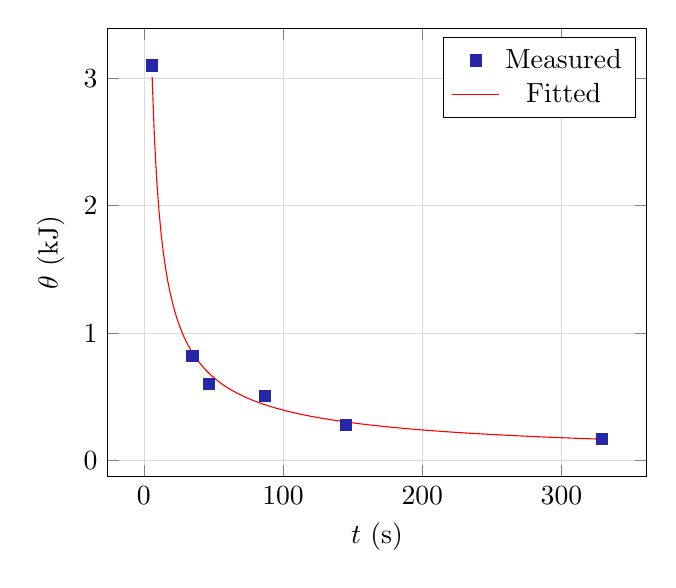
\begin{tikzpicture}
		\begin{axis}[
			xlabel={$t$ (s)},
			ylabel={$\theta$ (kJ)},
			xmin=6,
			xmax=329,
			grid=both,
			grid style={line width=0.2pt, draw=gray!30},
			%axis lines=left,
			enlarge x limits=0.1,
			enlarge y limits=0.1,
			legend style={at={(0.98,0.98)}, anchor=north east},
			]
			% Data points
			\addplot[only marks, mark=square*, mark size=2pt, color=blue!60!black!85] coordinates {
				(6, 3.10)
				(35, 0.82)
				(47, 0.60)
				(87, 0.51)
				(145, 0.28)
				(329, 0.17)
			};
			% Line plot
			\addplot[red, domain=6:329, samples=200] {10.93802*x^(-0.72)};
			% Legend
			\legend{Measured, Fitted}
		\end{axis}
	\end{tikzpicture}
	\hfill
	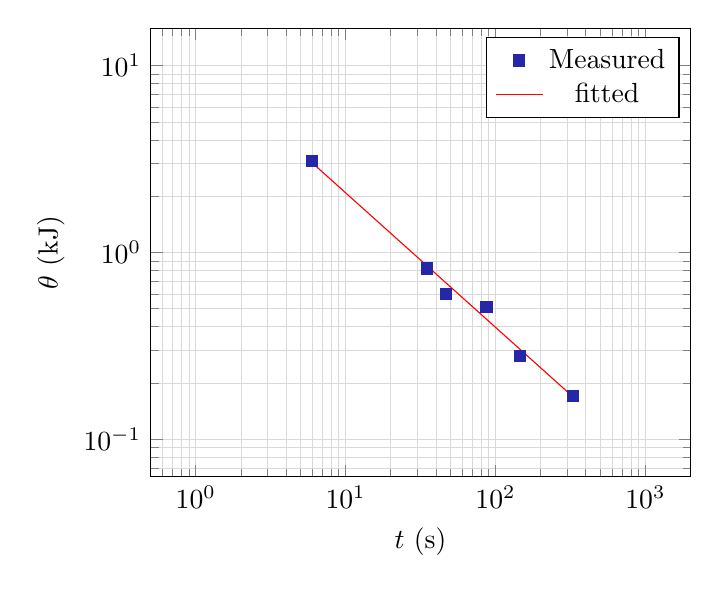
\begin{tikzpicture}
		\begin{loglogaxis}[
			xlabel={$t$ (s)},
			ylabel={$\theta$ (kJ)},
			xmin=1,
			xmax=1000,
			ymin=0.1,
			ymax=10,
			grid=both,
			grid style={line width=0.2pt, draw=gray!30},
			%axis lines=left,
			enlarge x limits=0.1,
			enlarge y limits=0.1,
			legend style={at={(0.98,0.98)}, anchor=north east},
			]
			% Original data points
			\addplot[only marks, mark=square*, mark size=2pt, color=blue!60!black!85] coordinates {
				(6, 3.10)
				(35, 0.82)
				(47, 0.60)
				(87, 0.51)
				(145, 0.28)
				(329, 0.17)
			};
			\addplot[red, domain=6:329, samples=200] {10.93802*x^(-0.72)};
			% Legend
			\legend{Measured, fitted}
		\end{loglogaxis}
	\end{tikzpicture}
    \caption{{\small A tikzpicture figure displaying the measured values (blue dots) (those in Table~\ref{t:heat}) for the quantity remaining heat at various times, along with the fitted power function $10938.02t^{-0.72}$ (continuous red).}\label{f:analysis_tikzpicture}}
\end{figure}
%
%
The relative error can be obtained through further analysis, i.e.,
%
\begin{equation}
    \frac{\|\hat{\mathbf{z}}-\mathbf{z}\|}{\|\mathbf{z}\|}\approx0.014.
\end{equation}
%
% Diagram ska ha storhet och enhet på axlarna (SI). Är det tex
% logaritmerade diagram ska de ha storhet (men inte enhet) på
% axlarna.
% Figurnummer och text ska stå under figur och hänga ihop på
% samma sida.
%
For those interested, there is a package in \LaTeXe\ for creating graphs directly in the source file. Check out
\href{https://www.overleaf.com/latex/examples/latex-figures-using-tikzpicture-pgfplots-and-overpic/dffvyqktbcwk}{https://www.overleaf.com/latex/examples/latex-figures-using-tikzpicture-pgfplots-and-overpic}.

\subsection{Subheading one if necessary}\label{s:resultsubsection1}
If you have one, you must have at least two (see below).

\subsubsection{Sub-subheading here if needed}
But if you have one, you must...

\subsubsection{Sub-subheading two under subheading}
...have at least one more.

\subsection{Subheading two}
This is on the same level as subheading~\ref{s:resultsubsection1}, indicating that there are at least two subheadings within the results section of this report.

%%%%%%%%%%%%%%%%%%%%%%%%%%%%%%%%%%%%%%%%%%%%%%%%%%%%%%%%%%%%%%
% - Discussion and Conclusions                             - %
%%%%%%%%%%%%%%%%%%%%%%%%%%%%%%%%%%%%%%%%%%%%%%%%%%%%%%%%%%%%%%
\newpage
\section{Discussion and Conclusions}

% Can be divided into separate chapters: "Discussion" and "Conclusions".
% Conclusions should be short and concise.
% Sometimes it is most appropriate to divide it into "Discussion" and "Conclusions and Future Work".

In this section, the results are discussed in a broader perspective and related to previous work, if applicable. Necessary conclusions are drawn to address the stated goals and the relevance of the results. Connect the conclusions to the established goals. Discuss sources of error and uncertainties. For example, it could be mentioned that ``the relative error of approximately 1.4\% suggests that the power function $10398.02t^{-0.72}$ represents the remaining heat with relatively good accuracy.''

It is also appropriate to conclude with suggestions and recommendations for further studies and investigations in the field. ``To better ensure the accuracy of the approximation, more data points are needed.'' Finally, it should be noted that the discussion, conclusions, and future studies can be divided into separate chapters if desired.

%%%%%%%%%%%%%%%%%%%%%%%%%%%%%%%%%%%%%%%%%%%%%%%%%%%%%%%%%%%%%%
% -                  References/Bibliography                - %
%%%%%%%%%%%%%%%%%%%%%%%%%%%%%%%%%%%%%%%%%%%%%%%%%%%%%%%%%%%%%%
\newpage
\bibliographystyle{unsrtnat}
\bibliography{references}

% In this section, you list the sources you have used in your work. Only include the most important references, and all references in the list must be cited in the text. The reference list should not include any "nice to have" references; only the ones the author has used. All references should be cited in the text.
% Note: Use original references. Avoid references to web pages as they may disappear/change, and remember to always include the date when the page was accessed in the reference.
%
% One of the most common ways is to write the author's name and the publication year of the reference - the so-called Harvard system.
% Example: ... also found by Charpak (1983).
% If there are two or more authors, you would write
% Two authors: ... also found by Charpak and Öqvist (1983).
% Multiple authors: ... also found by Charpak et al. (1983).
% ("et al." is Latin (et alii) and means "and others").
%
% Another way to cite a reference is to number the references in the order they appear in the text and sort the reference list in numerical order.
% Example: ... as found by Öqvist [3], and the reference Öqvist would then appear as number three in the reference list.
% A guide for references can be found here:
% https://www.ltu.se/ltu/lib/Skriva/Att-referera?l=en

\end{document}